\documentclass{article}
\usepackage[margin=1in]{geometry}
\usepackage{graphicx,caption,subcaption,xcolor,float,url,hyperref}
\captionsetup{font=small,labelfont=bf,justification=raggedright,singlelinecheck=false}
\pagestyle{empty}
\captionsetup[subfigure]{font=footnotesize,labelfont=normalfont,labelformat=parens,
  justification=centering,singlelinecheck=false,skip=3pt}
\newlength{\panelrowheight}
\newcommand{\figurepanel}[4]{%
  \begin{subfigure}[t]{#1}\centering
    \begin{minipage}[c][\panelrowheight][c]{\linewidth}\centering
      \includegraphics[pagebox=cropbox,width=\linewidth,height=\panelrowheight,keepaspectratio]{#2}%
    \end{minipage}
    \caption{#3}\label{#4}
  \end{subfigure}%
}
\begin{document}

\clearpage

\clearpage
\begin{figure}[H]
  \centering
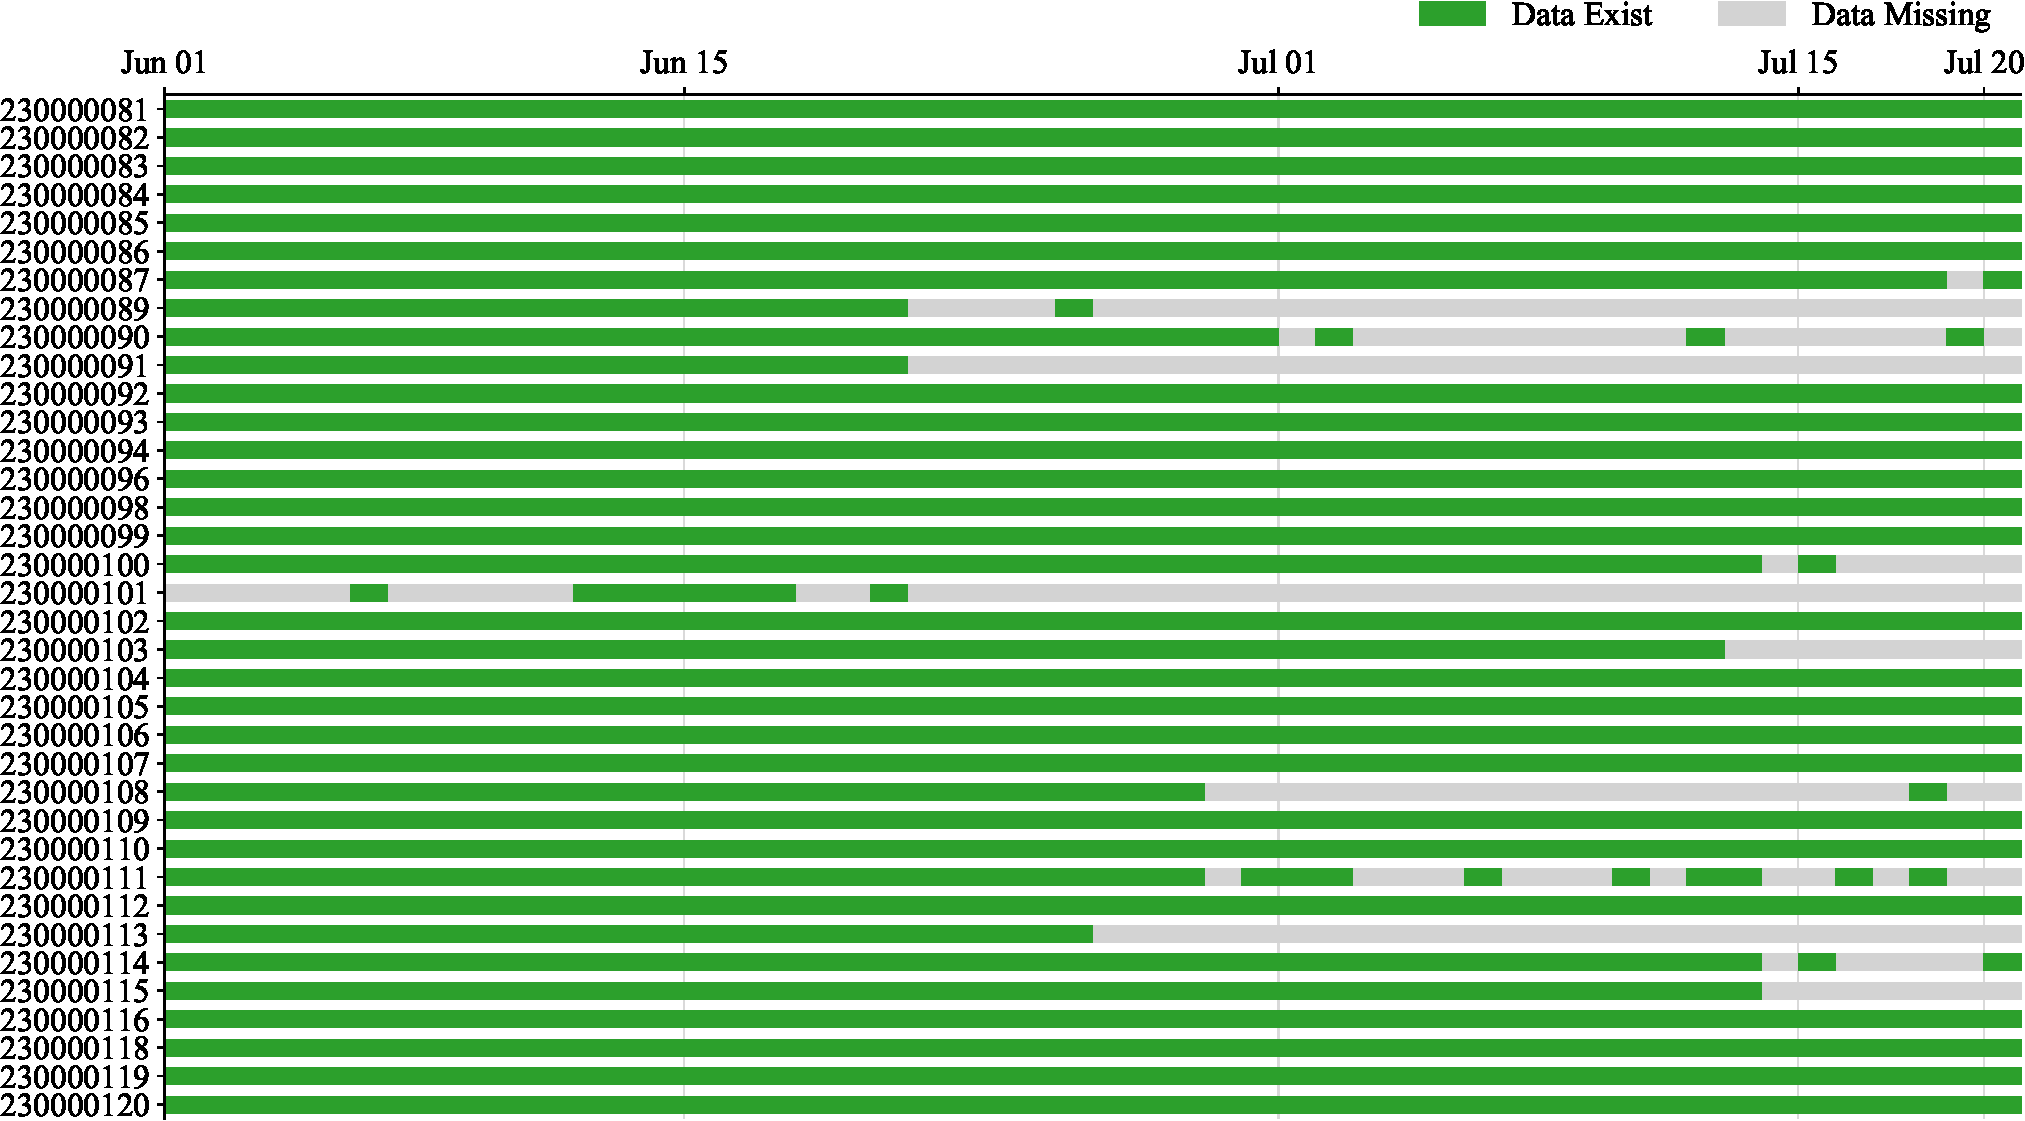
\includegraphics[pagebox=cropbox,width=\linewidth]{reference/fig3.pdf}
    \caption{\textbf{Raw-data availability by sensor and date.} Green represents periods with valid data, and gray represents periods with no data. A green cell indicates that all three components of the corresponding station were available on that date. Station-level availability for 1 June 2025 is resolved at five-minute intervals in the accompanying availability log.}
    \label{fig:data_availability}
\end{figure}
\clearpage
\begin{figure}[H]
  \centering
\setlength{\panelrowheight}{.321\linewidth}
\figurepanel{.193\linewidth}{reference/fig4-a.pdf}{\textcolor{blue}{Microseismic}}{fig:event_a}%
\hfill
\figurepanel{.193\linewidth}{reference/fig4-b.pdf}{\textcolor{blue}{Blasting}}{fig:event_b}%
\hfill
\figurepanel{.193\linewidth}{reference/fig4-c.pdf}{\textcolor{blue}{\scriptsize Small landslide}}{fig:event_c}%
\hfill
\figurepanel{.193\linewidth}{reference/fig4-d.pdf}{\textcolor{blue}{\scriptsize Mechanical mining}}{fig:event_d}%
\hfill
\figurepanel{.193\linewidth}{reference/fig4-e.pdf}{\textcolor{blue}{\scriptsize Transport vehicles}}{fig:event_e}
  \caption{\textcolor{blue}{\textbf{Examples of five event types after 1--20 Hz band-pass filtering.} Each column shows the waveform normalized to its own peak absolute amplitude, the 1--20 Hz time--frequency representation and the normalized STA/LTA characteristic function. The waveform time axis starts at the first sample of each window. The STA/LTA curve starts at the first sample with a complete 3 s long window. Panel (c) shows an external small-landslide example.}}
  \label{fig:waveform}
\end{figure}
\clearpage

\clearpage
\begin{figure}[H]
  \centering
\setlength{\panelrowheight}{.323\linewidth}
\figurepanel{.487\linewidth}{reference/fig6-a.pdf}{\textcolor{blue}{Raw three-component record}}{fig:raw_structure}%
\hfill
\figurepanel{.487\linewidth}{reference/fig6-b.pdf}{\textcolor{blue}{Classified blasting window}}{fig:event_structure}
  \caption{\textcolor{blue}{\textbf{Waveform examples from the released dataset.} Panel (a) shows an illustrative five-minute raw waveform segment recorded at station 230000081 on 1 June 2025, from \nolinkurl{230000081.20250601.000006000.DHE.miniseed}, \nolinkurl{230000081.20250601.000006000.DHN.miniseed} and \nolinkurl{230000081.20250601.000006000.DHZ.miniseed}. The traces are labelled by their miniSEED header channel codes. Panel (b) shows an illustrative filtered vertical-component blasting window from \nolinkurl{sensor_230000081_20250603T103254.752000_20250603T103257.320000.npy}. Shading marks the STA/LTA trigger interval. Both examples are sampled at 250 Hz and shown in instrument counts.}}
  \label{fig:data}
\end{figure}
\clearpage
\begin{figure}[H]
  \centering
\setlength{\panelrowheight}{.235\linewidth}
\figurepanel{.255\linewidth}{reference/fig7-a.pdf}{\textcolor{blue}{Five-class distribution}}{fig:five_class_counts}%
\hfill
\figurepanel{.255\linewidth}{reference/fig7-b.pdf}{\textcolor{blue}{Four-class distribution}}{fig:four_class_counts}%
\hfill
\figurepanel{.465\linewidth}{reference/fig7-c.pdf}{\textcolor{blue}{Chronological whole-day split}}{fig:classification_split}
\par\vspace{7pt}
\setlength{\panelrowheight}{.332\linewidth}
\figurepanel{.486\linewidth}{reference/fig7-d.pdf}{\textcolor{blue}{Feature-space projection}}{fig:feature_space}%
\hfill
\figurepanel{.486\linewidth}{reference/fig7-e.pdf}{\textcolor{blue}{Four-class test metrics}}{fig:classification_check}
  \caption{\textcolor{blue}{\textbf{Technical validation of the classified waveforms.} Panels (a) and (b) give the record counts for the five original labels and the four-class scheme, which combines microseismic and small-landslide records as natural slope events. Panel (c) shows the chronological whole-day split into 11,437 training, 4,165 validation and 2,020 test records. Panel (d) shows a t-SNE projection of 4,000 records using the fine-tuned CNN embeddings. Panel (e) gives precision, recall and F1-score for the CNN--Random Forest ensemble on the four-class test set, including the macro averages.}}
  \label{fig:Validation}
\end{figure}
\clearpage

\clearpage

\end{document}
